\chapter{Umsetzung}
\label{sec:Umsetzung}
In diesem Kapitel werden die einzelnen Schritte der Implementierung des Spielkonzepts beschrieben. Hierbei wird auf die unterschiedlichen Komponenten des Spiels eingegangen sowie auf die Schwierigkeiten, die bei der Implementierung aufgetreten sind.

\section{Implementierung des A* Algorithmus}
\label{sec:implementAStar}
\subsection*{Allgemein}
\begin{wrapfigure}{r}{7.5cm}
    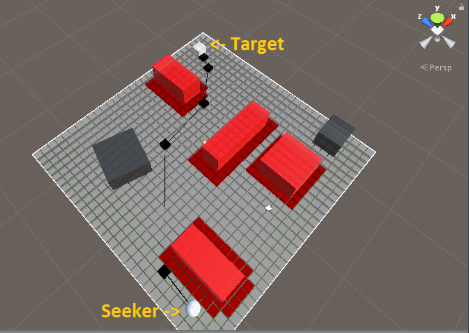
\includegraphics[width=7.5cm]{assets/aStarUnityImplementation.png}
    \caption{A* Implementation in Unity}
    \label{fig:aStarImplementationUnity}
\end{wrapfigure}
Die Implementierung des A* Algorithmus erfolgt in einem separaten Projekt, um mögliche Abhängigkeiten zu minimieren. Dieses Projekt ist in Abbildung \ref{fig:aStarImplementationUnity} zu sehen.
\begin{wrapfigure}{l}{4cm}
    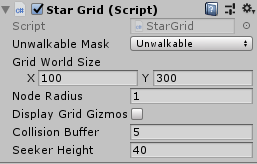
\includegraphics[width=4cm]{assets/aStarGridSettings}
    \caption{StarGrid Settings}
    \label{fig:aStarGridSettings}
\end{wrapfigure}
In der Grafik ist das Spielfeld, also das Grid mit seinen Nodes zu sehen, dort als graue oder rote Kacheln unter den Objekten dargestellt. Ein Node ist dementsprechend entweder als Pfad (grau) oder ein Hindernis (rot) gekennzeichnet.

Für das Bestimmen der Hindernisse auf dem Spielfeld wird die Funktionalität der Layers von Unity verwendet. Mit ihr lassen sich Spielobjekte logisch voneinander treffen. So sind die roten Quader auf dem selbst definierten Layer \textit{unwalkable}.

Wird das Spielfeld durch die \textit{StarGrid} Klasse generiert, kann gezielt nach den Hindernissen mit diesem Layer gesucht werden. Dann bekommen die Nodes, die entsprechende Eigenschaft ob sie begehbar oder nicht begehbar sind.

Damit dieses Skript im Kontext von Unity eingebunden werden kann, wird ein leeres \textit{GameObject} erstellt, was alle zum Algorithmus gehörenden Skripte zugewiesen bekommt. Dort lassen sich dann zum Beispiel Parameter wie die Größe des Grids, den Radius einen einzelnen Nodes oder ein Wert für einen Puffer setzen (siehe Abbildung \ref{fig:aStarGridSettings}). Der Puffer ist dann auf die Größe der Hindernisse drauf gerechnet, damit die Spielfigur einen größeren Abstand bei Verbeilaufen hat.

Sobald der A* den kürzesten Pfad berechnet hat bekommt er eine Liste mit Node-Position, welche dann verwendet werden, um die Spielfigur von Node zu Node laufen zu lassen aber auch den Pfad zu visualisieren. 

\subsection*{Binary-Min-Heap}
\begin{wrapfigure}[11]{R}{2in - .75\columnsep}
    \vspace{-\intextsep}
    \hspace*{-.75\columnsep}
    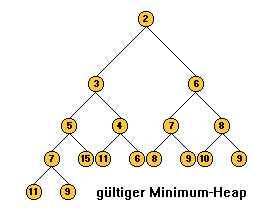
\includegraphics[width=4cm]{assets/heap_example.png}
    \caption{Binary-Min-Heap Beispiel}
    \label{fig:aStarHeap}
\end{wrapfigure}
Im Grundlagenkapitel \nameref{sec:fundamentalsA*} (\ref{sec:fundamentalsA*}) wird erläutert, das der A* Algorithmus eine \textit{Open List} verwendet, die benötigt wird, um alle Nodes zu speichern, die als möglicher Wegpunkt in Frage kommen. Da dessen Nodes häufig sortiert und aktualisiert werden muss, wird dafür ein Binary-Min-Heap als Priority Queue verwendet. Diese Datenstruktur kann effizient mit einem linearem Zeitaufwand von $O(n)$ erzeugt werden. Das Hinzufügen oder Entfernen von Elementen hat im schlimmsten Fall eine Laufzeit von $O(\log{n})$. Der Vorteil bei dieser Datenstruktur gegenüber einem herkömmlichen Arrays ist das \textit{in-place} Sortieren und wenn intern mit einem Array gearbeitet wird, ist der Speicherverbrauch gering und die Zugriffe sind schnell. Die Gesamtkomplexität für das Sortieren wäre im \textit{Worst-Case} $O(n*\log{n})$.

\subsection*{PathRequestManager}
Der \textit{PathRequestManger} ist eine Klasse, die implementiert wurde, um mehrere Wegberechnung nacheinander asynchronen abarbeiten zu lassen. Dabei verwaltet er alle Pfadanfragen und lässt alle nacheinander berechnen. Das sorgt dafür, dass der Spielfluss nicht durch das Blockieren des Hauptthreads unterbrochen wird.
\subsection*{Turret}
\begin{wrapfigure}[7]{L}{2in - .75\columnsep}
    \vspace{-\intextsep}
    \hspace*{-.75\columnsep}
    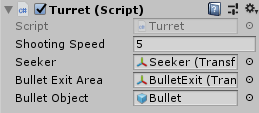
\includegraphics[width=4cm]{assets/aStarTurretSettings}
    \caption{PathRequestManager Settings}
    \label{fig:aStarTurretSettings}
\end{wrapfigure}
Für das im Kapitel \nameref{conclusion} (\ref{conclusion}) erwähnte Feature einer schießenden Einheit ist das \textit{Turret} Skript geschrieben worden. Dieses Skript wird einem \textit{GameObject} zugewiesen, welches dann auch im Spiel Projektile verschie\ss en soll. Als Projektil kann ein belibiges \textit{GameObject} verwendet werde. Sollte keines ausgewählt sein, wird ein Standard Projektil aus den Prefabs geladen. Wie in Abbildung \ref{fig:aStarTurretSettings} zu sehen, gibt es vier Parameter, welche angepasst werden können. Zum Einen sind das die Schussgeschwindigkeit, der Austrittsbereich, aus dem das Projektil geschossen wird und das eigentliche Projektil. Zum Anderen ist dort das Feld \textit{Seeker}, welche eine Referenz zur Spielfigur ist, also das Objekt auf das geschossen werden soll. Diese Komponente hat es noch nicht in das aktuelle Spiel geschafft, was aber mit dieser Klasse einfach nachzuholen ist.
\section{ImageTargets}
Wie im Kapitel \nameref{sec:rec_imageTargets} \ref{sec:rec_imageTargets} beschrieben, wurden vier unterschiedliche ImageTargets entworfen und in die Vuforia Datenbank geladen. Hierbei handelt es sich um Bilder von Gegenständen, die einem Studenten den Uni Alltag immer wieder erschweren. Bei den Gegenständen handelt es sich um die Mensa, Pizza, Bier und die Straßenbahn. Die Mensa steht für die komplizierte Platzsuche in einer überfüllten Mensa. Die Pizza repräsentiert das Ausweichessen, was es jeden Tag zu Hause gibt, wenn der Kühlschrank mal wieder leer ist. Das Bier steht für die Verlockung an einem sonnigen Abend den Stift fallen zu lassen und Bier zu trinken. Die Straßenbahn steht stellvertretend für die langen Anfahrtswege zur Uni.\\
Die ImageTargets haben sich im Laufe des Projekts den Anforderungen entsprechend verändert. Durch das Ranking in der Vuforia Datenbank stellte sich heraus, dass die ersten Entwürfe (siehe Abbildung \ref{fig:impl_imageTargets}) der ImageTargets einen schlechten Wiedererkennungswert aufwiesen. Aus diesem Grund mussten die Referenzbilder für die ImageTarget Detection überarbeitet werden. Durch die Anpassung der Bilder hat sich das Ranking durch die Vuforia Datenbank deutlich verbessert (siehe Abbildung \ref{fig:impl_vuforiaRanking}). Diese Verbesserung hat dazu beigetragen, dass die Bilder in der Anwendung auf auf größere Entfernungen besser erkannt und verfolgt werden konnten.
\begin{figure}[H]
    \centering
    \begin{subfigure}[b]{0.2\textwidth}
        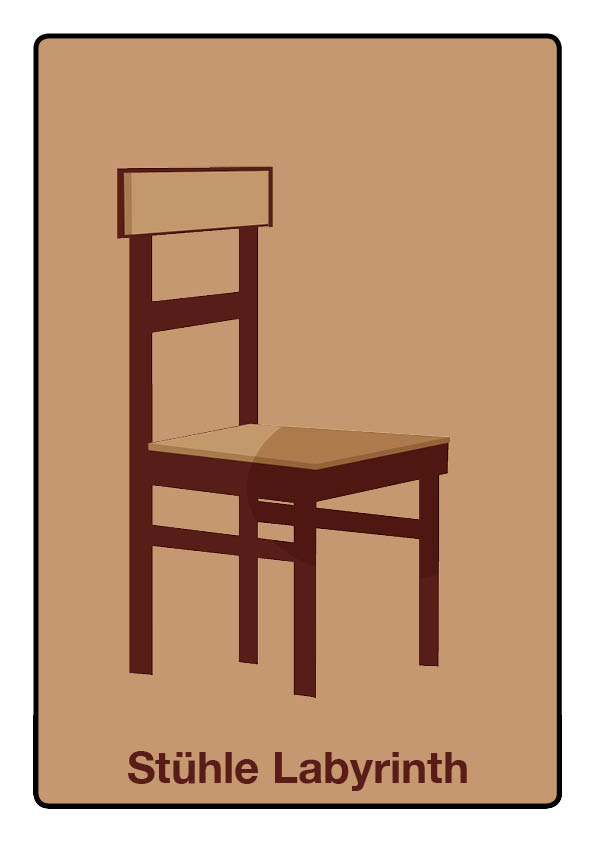
\includegraphics[width=\textwidth]{assets/mensa.jpg}
        \caption{Mensa Erstentwurf}
        \label{fig:oldMensa}
    \end{subfigure}
    ~
    \begin{subfigure}[b]{0.2\textwidth}
        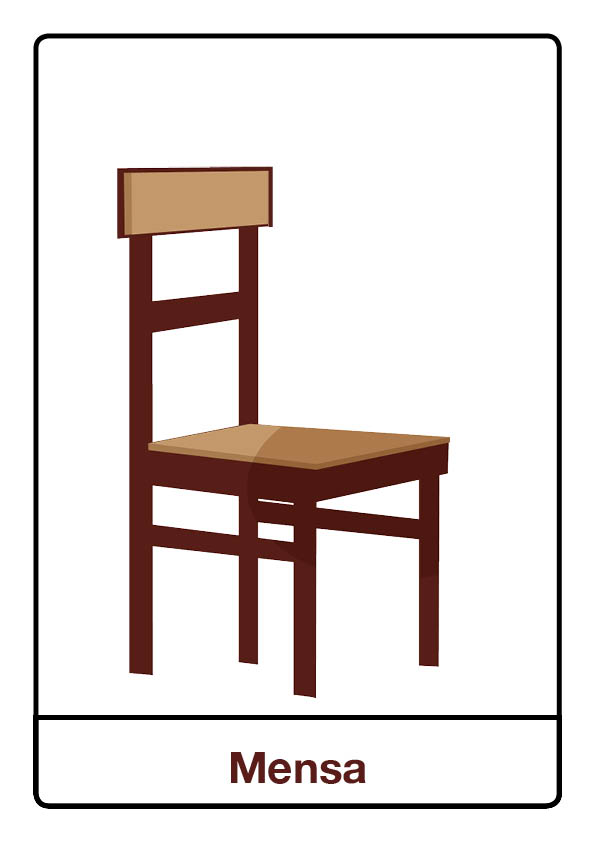
\includegraphics[width=\textwidth]{assets/mensa_new.jpg}
        \caption{Überarbeitete Mensa}
        \label{fig:newMensa}
    \end{subfigure}
    ~
    \begin{subfigure}[b]{0.2\textwidth}
        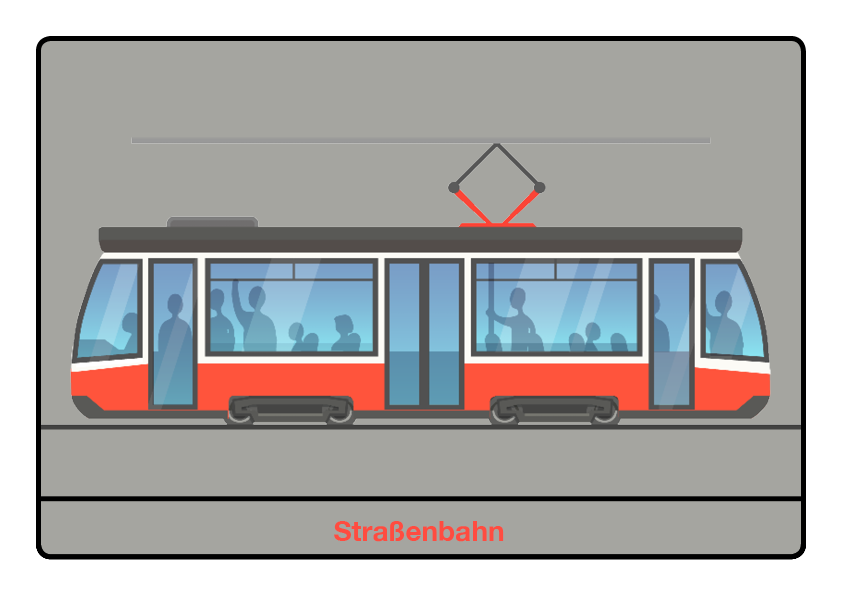
\includegraphics[width=\textwidth]{assets/tram.png}
        \caption{Tram Erstentwurf}
        \label{fig:oldTram}
    \end{subfigure}
    ~
    \begin{subfigure}[b]{0.2\textwidth}
        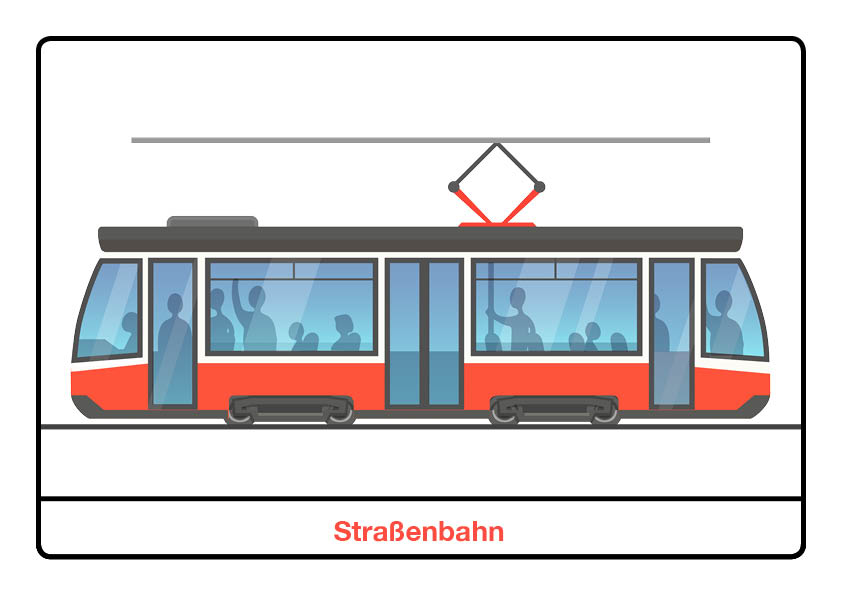
\includegraphics[width=\textwidth]{assets/tram_new.jpg}
        \caption{Überarbeitete Straßenbahn}
        \label{fig:newTram}
    \end{subfigure}
    \caption{Entwicklung der ImageTargets}\label{fig:impl_imageTargets}
\end{figure}

\begin{figure}[h]
        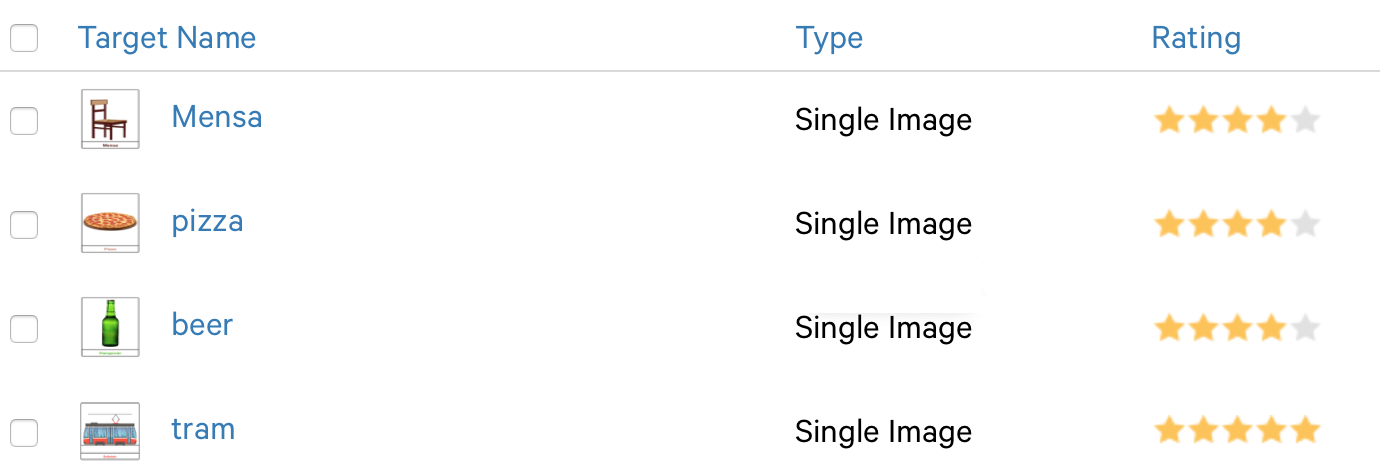
\includegraphics[width=\textwidth]{assets/vuforiaImageRanking}
        \caption{Vuforia Ranking}
        \label{fig:impl_vuforiaRanking}
\end{figure}

\section{Erkennung von Objekten}
Wie in Kapitel \ref{sec:vufObjRec} beschrieben müssen die eingescannten Objekte in eine Vuforia Datenbank importiert werden (siehe Abb. \ref{fig:vuforiaObjectDatabase}). Diese Datenbank wird im Vuforia Developer Portal zur Verfügung gestellt und ist mit wenigen Klicks eingerichtet. Diese Datenbank lässt sich für unterschiedliche Entwicklungsplattformen herunterladen. Unter anderem auch für die Unity IDE als package. Um die Objekte nun in der Unity Scene verwenden zu können, muss das Package per Import Package Funktion in Unity geladen werden.
\begin{figure}[h]
    \centering
    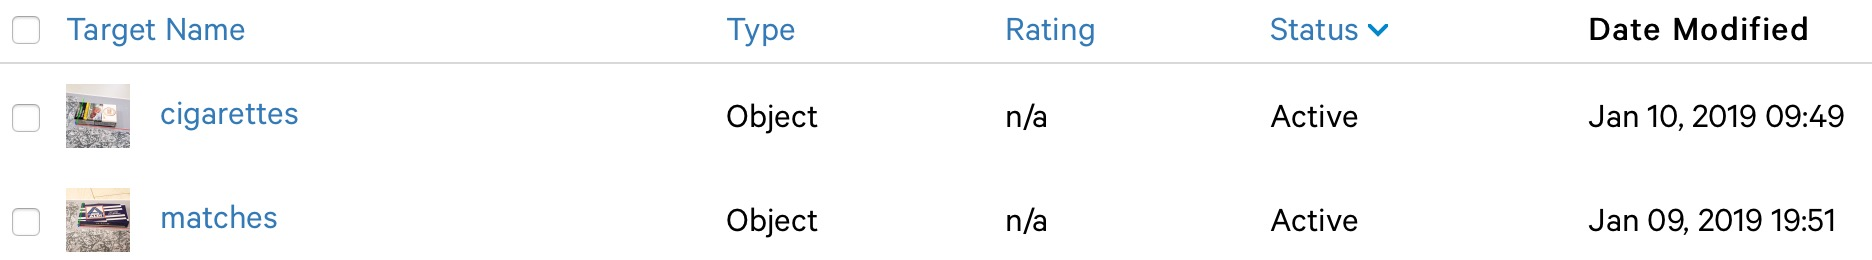
\includegraphics[width=\textwidth]{assets/vuforiaDataBase.jpeg}
    \caption{Vuforia Datenbank}\label{fig:vuforiaObjectDatabase}
\end{figure}\\
Vuforia bietet die Möglichkeit in Unity 3d Scan Objekte als Gameobjekt anzulegen. Bei dem angelegten Objekt kann nun die importierte Datenbank und das wiederzuerkennende Objekt ausgewählt werden. \\
In der Szene erscheint nun eine Bounding Box. Laut der Vuforia Dokumentation\cite{VufObjRec}  sollte die Bounding Box den Maßen des eingescannten Objektes entsprechen. Dies ist bei der Durchführung jedoch nicht der Fall gewesen. Die Objekte haben einen Nullpunkt. (siehe Abb. \ref{fig:matches}) Der Nullpunkt wird von der Schablone welche zum Einscannen genutzt wird, übernommen. Die Bounding Box bietet sich gut an, um Objekte auf dem eingescannten Objekt zu platzieren. Jedoch ist die Länge vom Nullpunkt bis zum Ende des Objektes nicht bekannt. Auch rechteckige Objekte werden durch eine quadratische Bounding Box dargestellt. Durch diesen Umstand kann keine präzise Bounding Box generiert werden, die das reale Objekt in der Scene widerspiegelt.\\
\begin{figure}[h]
    \centering
    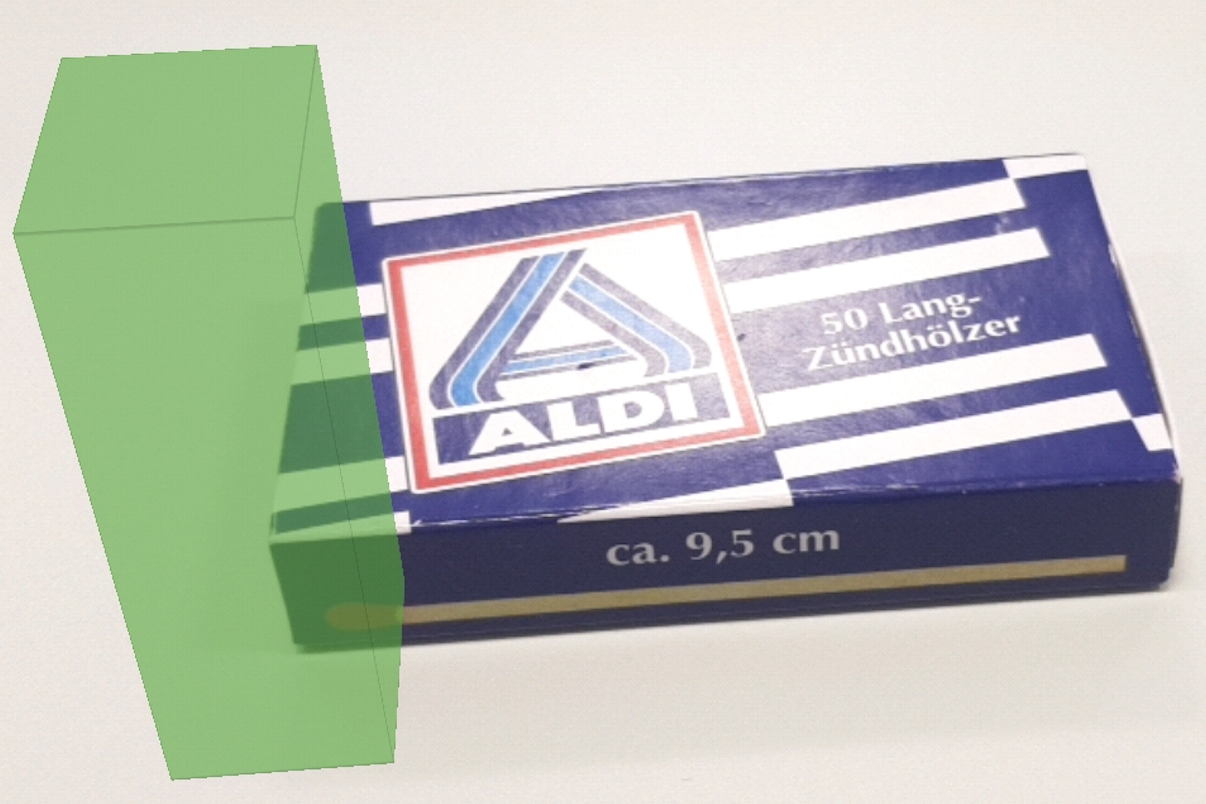
\includegraphics[width=0.5\linewidth]{assets/matches.png}
    \caption{Eingescanntes Objekt mit Nullpunkt}\label{fig:matches}
\end{figure}\\
Dem in der Scene befindlichen 3d Scan Game Object kann nun der \textit{unwalkable Layer} zugewiesen werden siehe \ref{sec:implementAStar} \nameref{sec:implementAStar}. Im Test reagierte der A* Algorithmus nicht auf die realen Objekte, da diese sich nicht auf der selben Ebene befinden wie das Spielfeld. Durch diesen Umstand haben wir den \textit{DefaultTrackableEventHandler} von Vuforia erweitert. Hierfür wurde ein eigenes Script implementiert, welches die eingescannten Objecte bei jedem Update auf die Position 0 der y-Achse transformiert. So wird sichergestellt, dass sich das reale Objekt und das Spielfeld auf der selben Ebene befinden. Das reale Objekt wurde daraufhin von den Nodes des A* Grids als unwalkable erkannt. \\
Um die Objekte in die Scene des Spielers zu integrieren muss sich die Kamera exakt über dem Spielfeld befinden. Eine Third Person Ansicht ist nicht möglich, da die erkannten Objekte von der Position der Kamera ausgehen. Steht die Kamera Beispielsweise auf xyz(0,-20, -20), erhält das gescannte Objekt ebenfalls diese Koordinaten. Wird das Objekt in der realen Welt bewegt, verändern sich die Koordinaten, allerdings ausgehend von der Kamera Position. Durch diesen Umstand muss die Kamera exakt in der Mitte des Spielfelds befinden, damit die realen Objekte ausgehend von diesem Punkt platziert werden können.

\section{UI}
Wie in Abbildung \ref{fig:uiElements} zu sehen ist, besteht das User Interface für die RunnAR Anwendung aus zwei unterschiedlichen Ansichten. Zum Einen ist in Abbildung \ref{fig:uiMenu} das Startmenü zu sehen. Hierbei hat der Nutzer die Möglichkeit die Anwendung zu verlassen indem der Exit Button geklickt wird, oder das Spiel kann durch den Start Button gestartet werden. Zum Anderen besteht die Anwendung aus der Spielansicht (siehe Abbildung \ref{fig:uiGame}). Die Spielansicht beinhaltet einen Replay Button, einen Timer sowie den Spieler und alle Interaktionselemente für den Spieler. Durch den Replay Button lässt sich der derzeitige Spielstand zurücksetzen und von Neuem beginnen. Der Timer läuft runter von 90 Sekunden. Ist die Zeit abgelaufen ist die Spielrunde beendet. Das UI der Anwendung befindet sich in einem prototypischen Zustand, der eine einfache Bedienung ermöglicht.

\begin{figure}[H]
    \centering
    \begin{subfigure}[b]{0.3\textwidth}
        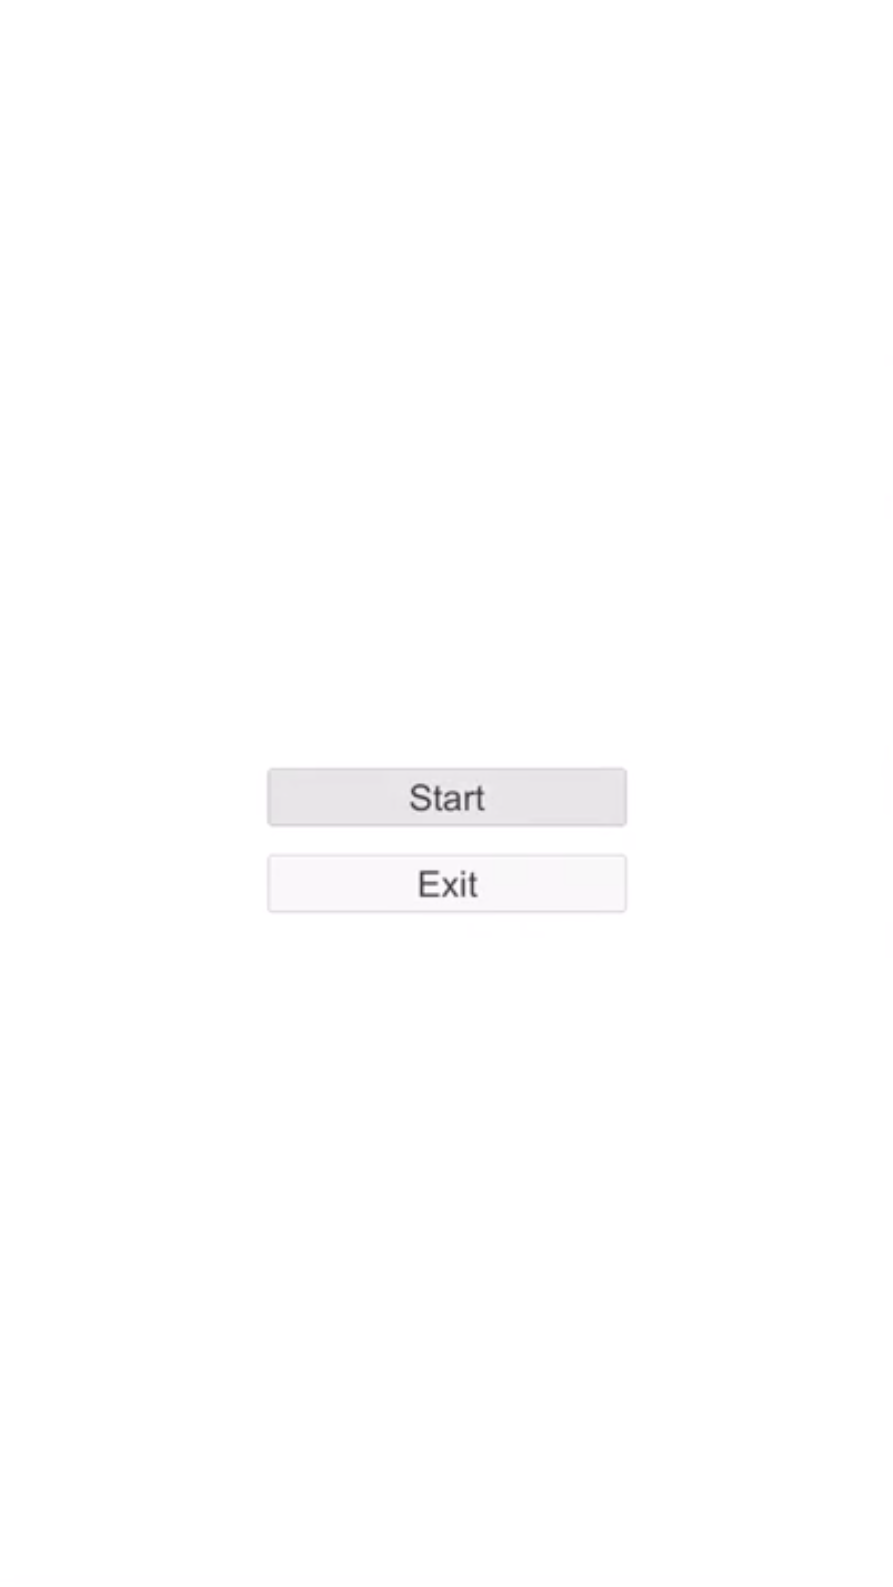
\includegraphics[width=\textwidth]{assets/uiMenu}
        \caption{UI Menüansicht}
        \label{fig:uiMenu}
    \end{subfigure}
    ~
    \begin{subfigure}[b]{0.3\textwidth}
        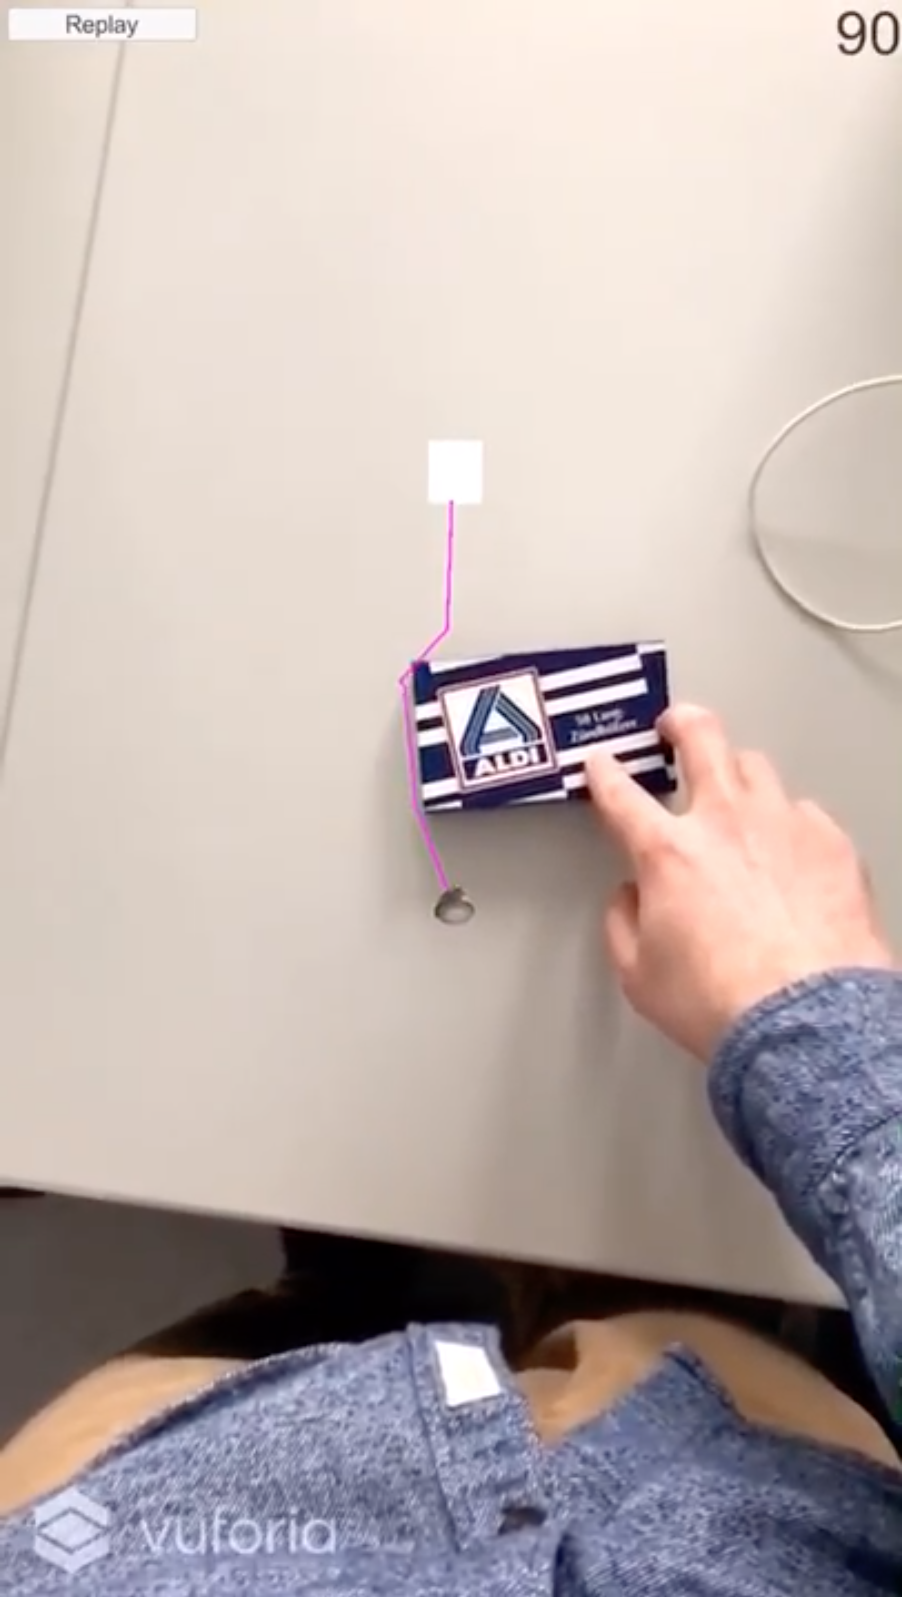
\includegraphics[width=\textwidth]{assets/uiGame}
        \caption{UI Spielansicht}
        \label{fig:uiGame}
    \end{subfigure}
    \caption{User Interface Elemente}\label{fig:uiElements}
\end{figure}

